\chapter*{Introduction}\phantomsection\addcontentsline{toc}{chapter}{Introduction}

\section*{Credits}\phantomsection\addcontentsline{toc}{section}{Credits}

\section*{A Short Summary}\phantomsection\addcontentsline{toc}{section}{A Short Summary}

\chapter*{Optional: Private, the Mystery}\phantomsection\addcontentsline{toc}{chapter}{Optional: Private, the Mystery}

\section*{Private's Character Development (Ideas)}\phantomsection\addcontentsline{toc}{section}{Private's Character Development (Ideas)}
\begin{itemize}
	\item \textbf{Hexblade Curse}\\
	When Private misses an attack on a creature within 30ft of him, he will curse at the target that he missed, using some even for him unknown language. When the creature dies he will feel invigorated as he gains HP (level + Charisma Modifier - minimum of 1). Therefore, Private realizes that he can curse his target.
	\item \textbf{Hex Warrior}\\
	When Private uses a martial or simple weapon that does not have the two-handed property and does damage to any creature, he realizes that it does much more damage than it usually would.
	\item \textbf{Investment of the Chain Master}\\
	As soon as Private finds a familiar he realizes that it has additional features
	\item \textbf{Pact of the Chain}\\
	As soon as Private finds a familiar he realizes that it has additional features
	\item \textbf{Spell Sniper}
	If Private hits 5 consecutive spell attacks or a creature that is hiding in half or three-quarter cover, he will wonder why his accuracy is greatly improved learning that he is a Spell Sniper.
	\item \textbf{Spells}
	As a Warlock Private can cast different spells. However, as he is not aware of those he will realize, most often just by chance, that he can use those, either by certain circumstances or by different opportunities in the game world.
	\begin{itemize}
		\item \textcolor{titlered}{\textbf{Mage Hand}}\\
		During the random quest encounter at the lake in the Central Park, Private will save a gosling by casting Mage Hand.
		\item \textcolor{titlered}{\textbf{Armor of Agathys (Glacial Wall)}}\\
		When Private is stuck in the powdered snow in the polar bear habitat for more than one turn, and successfully frees himself from this predicament he realizes that some snow particles are floating around him, forming a kind of shield or aura. This effect gives Private 5 Temporary HP and each creature that attacks him with a melee attack takes 5 cold damage. After this situation Private gains the ability to cast "Glacial Wall", which is indifferent from the effect of "Armor of Agathys".
		\item \textcolor{titlered}{\textbf{Hex (Weakening)}}\\
		When one creature is successful on three ability saving throw checks within one round of combat, Private lashes out with unknown incantations, cursing the target. With this he successfully casts Hex with the targeted ability to be the last ability save that the creature was able to resolve.\\
		A creature under the influence of this spell also takes additional 1d6 necrotic damage whenever it is hit by an attack made by Private.\\
		When the target dies the curse can be switched to another creature within range as a Bonus Action.
		\item \textcolor{titlered}{\textbf{Find Familiar}}\\
		After unlocking the food storage a small animal will approach the group of adventurers asking for food. If the animal is given food it will offer to become the loyal familiar of private, such Private gins the ability to cast Find Familiar.
		\item \textcolor{titlered}{\textbf{Darkness}}\\
		Private can learn this spell when the Dark Forest puzzle is solved.
		\item \textcolor{titlered}{\textbf{Invisibility}}\\
		Private can learn this spell from the chameleon in the Reptile House.
	\end{itemize}
\end{itemize}

\adventurepart{Setting: Central Park Zoo}{}{}{}{}{}{}{}{}

\onecolumn
\begin{multicols}{2}
\DndDropCapLine{W}{\entryfont elcome to the bustling heart of Manhattan, New York City, where towering skyscrapers and the urban jungle of Central Park meet. Hidden within this iconic park lies the Central Park Zoo, a world of wonder and wildlife tucked amidst the urban sprawl. This adventure begins right here, in the vibrant and lively zoo, a sanctuary for animals and the stage for your thrilling escapades.}

{\entryfont As you step through the zoo's main gate, the noise of Manhattan fades into the background, replaced by the hum of life within the zoo. The cheerful chatter of visitors mingles with the roars, chirps, and splashes of its residents, forming a symphony of sounds that sets the stage for your journey. Meandering pathways lead you through diverse habitats, each brimming with character - from the icy Arctic refuge of the polar bears to the lush greenery of the lemurs' domain. Vibrant flower beds, shady trees, and scattered benches provide picturesque spots to pause and soak in the surroundings.

This adventure takes place entirely within this bustling haven, where every enclosure, path, and corner holds the potential for excitement and intrigue. At its heart lies the Penguin Habitat, a hub of activity and the headquarters for your daring exploits. Your story begins as the penguins, masters of strategy and mischief, set the stage for an unforgettable tale of teamwork, courage, and ingenuity.}

\section*{Central Park Zoo Map}\phantomsection\addcontentsline{toc}{section}{Central Park Zoo Map}
{\entryfont Your adventure unfolds within the carefully crafted environment of the Central Park Zoo, and the map provided will serve as your indispensable guide. This map highlights key locations such as the Penguin Habitat, Flamingo Habitat, and the bustling Main Gate, ensuring that you can navigate the zoo's myriad paths with ease. Each habitat has its own unique charm and challenges, offering opportunities for exploration, problem-solving, and unexpected encounters.

Whether plotting your next move from the comfort of the Souvenir Shop or investigating the secrets of the Reptile House, the map will help you visualize and immerse yourself in the vibrant world of the zoo. Keep it close at hand, as it will be your ally in uncovering the many surprises this adventure has to offer.}
\end{multicols}
\begin{tikzpicture}[overlay, remember picture]
	\node[yshift=-3.75cm] at (current page.center){%
		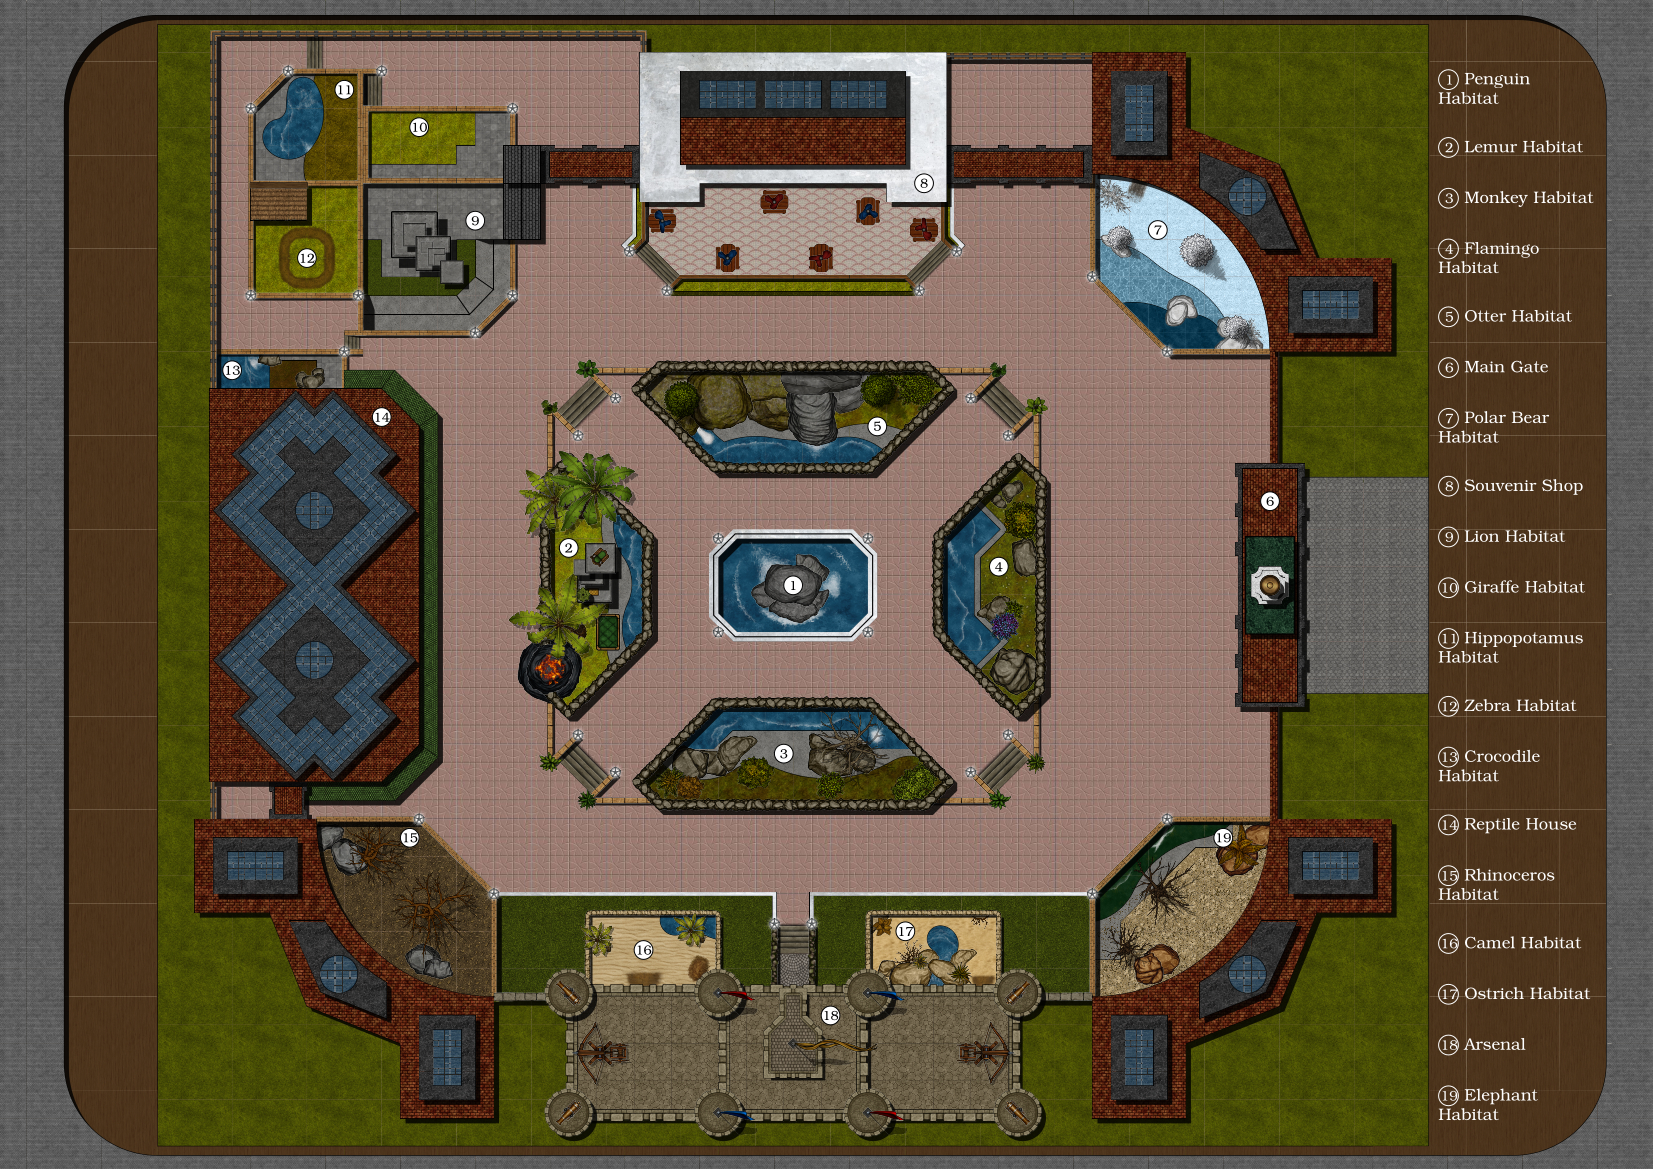
\includegraphics[width=0.95\paperwidth]{../maps/Central_Park_Zoo/map_Central_Park_Zoo.jpg}%
	};%
\end{tikzpicture}
{\vspace*{14.5cm}\hfill\\\footnotesize \textit{* The map provided is a creative amalgamation based on various interpretations of the Central Park Zoo. It is not an exact replica but is designed to represent the zoo's most recognizable features for narrative and game-play purposes.}}

\twocolumn

\adventurepart{Running the One-Shot}{}{}{}{}{}{}{}{}

\chapter*{A Quiet Morning}\phantomsection\addcontentsline{toc}{chapter}{A Quiet Morning}
\DndDropCapLine{A}{\entryfont s the first light of dawn creeps over the skyline of New York City, the tranquil setting of Central Park Zoo is aglow with the promise of a new day. As the bells of the Central Park Zoo chime to signal the official opening of the day, a sense of unease hangs heavy in the air. The wrought iron gates, adorned with intricate animal motifs, stand ajar, welcoming the non-existent throngs of visitors who should be streaming in. Yet, eerily, the pathways lie empty, devoid of the usual chatter and excitement.\\}

{\entryfont \paragraph*{A Welcome Tranquillity}
Skipper, Kowalski, Rico, and Private, the quartet of penguins known for their daring escapades and ingenious schemes, find themselves oddly content in the absence of the usual noisy visitors and screaming children.

While Rico diligently tinkers away, perfecting his craft of creating explosions with a determined gleam in his eye, Kowalski furiously scribbles notes, engrossed in his latest research endeavour. His musings are bound to culminate in another of his spectacular inventions, destined, no doubt, to crash or explode in a most spectacular fashion.

Meanwhile, Private, the gentlest soul among them, can't help but feel a pang of sadness at the deserted zoo. His heart aches for the laughter of children, the joyous squeals that once filled the air. Yet, even in his melancholy, he remains steadfast by his comrades' side.

And there's Skipper, perched nonchalantly on an inflatable rubber island, relishing the simple pleasure of a meal of fresh fish. With a contented sigh, he watches the sunlight dance across the tranquil waters, savouring the peace - wait fish? \textbf{FISH!}\\}

{\entryfont \paragraph*{A Stark Realization}
His beak opens in surprise as he scans the empty expanse of the once-bustling enclosure. The absence of their human caretakers dawns upon him, and with it, the stark realization that the zoo's larders remain untouched. There is no fish. No food at all. The tranquillity of the morning shattered by the pang of hunger, Skipper's gaze shifts to his comrades. Without a word exchanged, a silent agreement passes between them - \textbf{Operation: Search for Food} is under-way.}

\subsection*{Optional: Agent Ringtail}
{\entryfont As the penguins ready themselves, their preparations are interrupted by an unexpected sight in their midst. King Julien, accompanied by his loyal followers Mort and Maurice, scours the penguin's habitat and base in search of sustenance. Initially, Skipper's irritation flares at the intrusion, but Kowalski interjects with a surprising perspective. He points out that in their quest for food, having additional pairs of eyes and, more importantly, hands with opposable thumbs could prove to be a considerable advantage. Reluctantly, Skipper acquiesces, recognizing the potential benefits of an alliance with "Ringtail" and his cohorts for their mission. With a nod of agreement, the penguins and their unlikely allies set out together, united in their common goal of survival amidst the abandoned zoo.}

\begin{tikzpicture}[overlay, remember picture]
	\node[xshift=3.25cm, yshift=2.75cm] at (current page.center){%
		
\includegraphics[height=1.2\paperheight]{Penguins_side.png}%
	};%
\end{tikzpicture}

\chapter*{Operation: Search for Food}\phantomsection\addcontentsline{toc}{chapter}{Operation: Search for Food}
\subsubsection*{Starting Point: Penguin Habitat}
{\entryfont The players find themselves in the familiar confines of their own \inTextCircled[10]{1}{8} Penguin Habitat, where the rays of sunlight cast a golden hue over the zoo.}
\subsubsection*{Goal: Find Sustenance}
{\entryfont Their primary objective is clear: to secure food for themselves and their fellow zoo inhabitants. With the zoo's storage, nestled within the \inTextCircled[10]{8}{8} Souvenir Shop, rumoured to hold provisions, it becomes their initial target. Yet, the players also recognize the potential for sustenance scattered throughout the vast expanse of the zoo grounds. (The number of rations a certain sustenance item provides is always stated)}

\section*{At the Gates of FISH}\phantomsection\addcontentsline{toc}{section}{At the Gates of Fish}

\section*{Zoo Trip}\phantomsection\addcontentsline{toc}{section}{Zoo Trip}

\subsection*{\inTextCircled[10]{1}{10} Penguin Habitat}

\subsection*{\inTextCircled[10]{2}{10} Lemur Habitat}

\subsection*{\inTextCircled[10]{3}{10} Monkey Habitat}

\subsection*{\inTextCircled[10]{4}{10} Flamingo Habitat}
\textbf{\textit{Generator Location}}
\begin{DndReadAloud}
	The Flamingo Habitat, usually a vibrant sanctuary, now feels strangely subdued. The shallow pond at its center is murky and stagnant, its usual clarity replaced by a greenish haze. Restless flamingos cluster along the edges, avoiding the water entirely. Overgrown reeds partially obscure fountains that have fallen silent, their inactivity mirroring the habitat's sombre atmosphere. The air carries a faint smell of algae, hinting at the effects of the non-functioning generator.
\end{DndReadAloud}

\paragraph*{Enabling the Generator}
{\entryfont The generator for the Flamingo Habitat is located inside a small maintenance shed near the pond, partially obscured by reeds and vines. The door to the shed is locked and rusted shut, requiring a \textbf{Strength Check (DC 14)} to force open. Once inside, the generator is visible but submerged in several inches of water, rendering it inoperable in its current state.

To enable the generator, the players must remove the water from the shed. This can be achieved in a variety of ways:

\begin{itemize}
	\renewcommand\labelitemi{\textbf{\textbullet}}%
	\item \textbf{Using Tools or Magic}\\
	Players can use buckets, other creative tools found in their inventory, or a spell like Shape Water to remove the water.
	\item \textbf{Repairing the Drainage System}\\
	A \textbf{DC 15 Investigation Check} reveals a clogged drainage pipe at the back of the shed. Clearing the pipe (requiring a \textbf{Sleight of Hand (DC 13)} or Dexterity-based tool proficiency) allows the water to drain away.
\end{itemize}
Once the water is removed and the generator is dry, a quick lever pull reactivates it, sending a hum of power through the habitat. The fountains spray more forcefully, and the flamingos let out a chorus of celebratory honks, signaling success.}

\subsection*{\inTextCircled[10]{5}{10} Otter Habitat}
{\entryfont Players encounter Marlene, a spirited and agile otter with a playful gleam in her eye. Eager for entertainment in the desolate zoo, Marlene challenges the group to an \textbf{Acrobatic Contest}, her favourite pastime. In order to take part the group must wager an item of their choice - worth at least 10gp. 

Marlene, with her natural affinity for acrobatics, enjoys the advantage of both skill and experience. Her nimble movements and confident demeanour give her an edge, represented by a substantial +5 bonus to her Acrobatics skills and advantage on the roll.

If at least one player manages to surpass Marlene's impressive performance, the group is awarded one fish (one ration) as a token of their achievement. Should more than half of the group outshine the otter in the acrobatic display, an additional fish (one ration) is added to their prize. However, should the group falter and fail to best Marlene, the item provided to partake in the contest is forfeited.}

\subsection*{\inTextCircled[10]{6}{10} Main Gate}
\begin{DndReadAloud}
	The Main Gate of the zoo stands as a grand, welcoming archway adorned with intricate ironwork depicting animals in playful poses. The sturdy, dark-green bars glint faintly in the light, a testament to both their age and craftsmanship. Beyond the arch, a spacious plaza stretches out, paved with smooth, weathered stone tiles. Benches and flower beds line the edges, offering visitors a charming place to rest beneath the shade of towering oak trees.

	To the side of the plaza, a small ticket office sits nestled against the wall, its windows covered with faded posters advertising past zoo events. The wooden door to the office is slightly ajar, revealing a cluttered interior filled with stacks of old flyers, a dusty desk, and a locked medical cabinet tucked into the corner. Nearby, a bulletin board hangs on the wall, pinned with colourful zoo maps and reminders of rules for visitors. The faint scent of popcorn lingers in the air, a remnant of bustling crowds that pass daily through this lively entrance.
\end{DndReadAloud}

{\noindent\entryfont Aside from the medical cabinet containing the quest-item "Shot against Brown Spots," the party can also find a discarded sandwich tucked under a bench, providing 2 rations, and a map with annotations marking the placement of generators throughout the zoo. However, the map is buried beneath a pile of old flyers and clutter, requiring a successful \textbf{DC 16 Investigation Check} to uncover.

Perched atop the arch of the Main Gate, a small hippo plushy lies abandoned, its soft, round form visible to anyone who looks closely. A successful \textbf{Perception Check (DC 12)} reveals the plushy from below, drawing the party's attention to its unusual resting place. Reaching it requires climbing the gate. A player must succeed on an \textbf{Athletics (DC 12) or Acrobatics (DC 14) Check} to scale the gate safely.}

\subsection*{\inTextCircled[10]{7}{10} Polar Bear Habitat}
\textbf{\textit{Generator Location}}\\
% Monster Stat-Block
\begin{DndMonster}[width=0.5\textwidth - 4pt]{Ted (Polar Bear)}
	\DndMonsterType{Large Beast, unaligned}

	% If you want to use commas in the key values, enclose the values in braces.
	\DndMonsterBasics[
		armor-class = {14 (Natural Armor)},
		hit-points  = {\DndDice{8d10 + 24}},
		speed       = {40 ft., swim 30 ft.},
	]

	\renewcommand{\AbilityScoreSpacer}{~}

	\DndMonsterAbilityScores[
		str = 20,
		dex = 10,
		con = 16,
		int = 2,
		wis = 13,
		cha = 7,
	]

	\DndMonsterDetails[
		%saving-throws = {Str +0, Dex +0, Con +0, Int +0, Wis +0, Cha +0},
		skills = {Perception +3},
		%damage-vulnerabilities = {cold},
		damage-resistances = {cold},
		%damage-immunities = {cold},
		senses = {passive Perception 13},
		%condition-immunities = {frightened, poisoned, prone},
		languages = {Common},
		challenge = 5,
	]

	\DndMonsterAction{Keen Smell}
	The bear has advantage on Wisdom (Perception) checks that rely on smell.

	\DndMonsterAction{Snow Hide}
	While the polar bear is in a snowy environment it gets a +2 to AC.
	
	\DndMonsterSection{Actions}
	\DndMonsterAction{Multiattack}
	The bear makes two attacks: one with its bite and one with its claw.   

	\DndMonsterAttack[
		name=Bite,
		distance=melee, % valid options are in the set {both,melee,ranged},
		%type=weapon, %valid options are in the set {weapon,spell}
		mod=+7,
		reach=5,
		%range=20/60,
		targets=one target,
		dmg={\DndDice{1d8 + 5}},
		dmg-type=piercing,
		%plus-dmg=,
		%plus-dmg-type=,
		%or-dmg=,
		%or-dmg-when=,
		%extra={},
	]
	
	\DndMonsterAttack[
		name=Claws,
		distance=melee, % valid options are in the set {both,melee,ranged},
		%type=weapon, %valid options are in the set {weapon,spell}
		mod=+7,
		reach=5,
		%range=20/60,
		targets=one target,
		dmg={\DndDice{2d6 + 5}},
		dmg-type=slashing,
		%plus-dmg=,
		%plus-dmg-type=,
		%or-dmg=,
		%or-dmg-when=,
		%extra=,
	] 
\end{DndMonster}

\subsection*{\inTextCircled[10]{8}{10} Souvenir Shop and Café}

\subsection*{\inTextCircled[10]{9}{10} Lion Habitat}
\textbf{\textit{Generator Location}}\\
% Monster Stat-Block
\begin{DndMonster}[width=0.5\textwidth - 4pt]{Alex (Lion)}
	\DndMonsterType{Large Beast, unaligned}

	% If you want to use commas in the key values, enclose the values in braces.
	\DndMonsterBasics[
		armor-class = {15 (Natural Armor)},
		hit-points  = {\DndDice{8d10 + 8}},
		speed       = {50 ft.},
	]

	\renewcommand{\AbilityScoreSpacer}{~}

	\DndMonsterAbilityScores[
		str = 17,
		dex = 15,
		con = 13,
		int = 3,
		wis = 12,
		cha = 8,
	]

	\DndMonsterDetails[
		%saving-throws = {Str +0, Dex +0, Con +0, Int +0, Wis +0, Cha +0},
		skills = {Perception +3, Stealth +6},
		%damage-vulnerabilities = {cold},
		%damage-resistances = {cold},
		%damage-immunities = {cold},
		senses = {passive Perception 13},
		%condition-immunities = {frightened, poisoned, prone},
		languages = {Common},
		challenge = 3,
	]

	\DndMonsterAction{Keen Smell}
	The lion has advantage on Wisdom (Perception) checks that rely on smell.
	
	\DndMonsterAction{Pounce}
	If the lion moves at least 20 ft. straight toward a creature and then hits it with a claw attack on the same turn, that target must succeed on a DC 13 Strength saving throw or be knocked prone. If the target is prone, the lion can make one bite attack against it as a bonus action.
	
	\DndMonsterAction{Running Leap}
	With a 10-foot running start, the lion can long jump up to 25 ft..
	
	\DndMonsterSection{Actions}   

	\DndMonsterAttack[
		name=Bite,
		distance=melee, % valid options are in the set {both,melee,ranged},
		%type=weapon, %valid options are in the set {weapon,spell}
		mod=+5,
		reach=5,
		%range=20/60,
		targets=one target,
		dmg={\DndDice{1d8 + 3}},
		dmg-type=piercing,
		%plus-dmg=,
		%plus-dmg-type=,
		%or-dmg=,
		%or-dmg-when=,
		%extra={},
	]
	
	\DndMonsterAttack[
		name=Claw,
		distance=melee, % valid options are in the set {both,melee,ranged},
		%type=weapon, %valid options are in the set {weapon,spell}
		mod=+8,
		reach=5,
		%range=20/60,
		targets=one target,
		dmg={\DndDice{1d6 + 3}},
		dmg-type=slashing,
		%plus-dmg=,
		%plus-dmg-type=,
		%or-dmg=,
		%or-dmg-when=,
		%extra={},
	]
\end{DndMonster}

\subsection*{\inTextCircled[10]{10}{10} Giraffe Habitat}
\begin{DndReadAloud}{}
	As you approach the Giraffe Habitat, a nervous voice calls down from above. Towering over the fence, a giraffe with a perpetually worried expression cranes his neck toward you.

	\textit{"Oh no, oh no, oh no!"} he frets, awkwardly shifting his long legs. \textit{"It's happened again! Another brown spot! Look at it - it's enormous!"} He stretches his neck further to reveal an entirely normal giraffe marking.

	\textit{"Please, you have to help me! I need my 'Shot against Brown Spots'. It's the only thing that works. You'll find it in the zoo somewhere - I just know it! But hurry! Who knows how many more might appear!”}

	Melman lowers his head expectantly, his wide eyes pleading as he waits for your response.
\end{DndReadAloud}

\begin{DndQuestHook}[width=0.5\textwidth - 4pt]{Brown Spots}
	\DndQuestHookBasics[
		location = {Giraffe Habitat},
		quest-giver = {Melman, the Giraffe},
		objective = {Find the medicine (\textit{"Shot against Brown Spots"})},
	]
	
	{\noindent\entryfont The medicinal vial can be found at the \inTextCircled[10]{6}{8} Main Gate, stored in a small locked medical cabinet in the corner of the ticket office. The cabinet has a combination lock with three dials, each bearing a series of numbers (0–9). To open the lock, players must find clues scattered in the ticket office area:
	\begin{itemize}
		\item A faded poster of the zoo opening hours with the 8 highlighted, giving the first number.
		\item A calendar with an animal-themed pattern where giraffes are prominently marked on the 9th day of the month, providing the second digit.
		\item A price chart showing the cost of a child's ticket as 5 dollars, revealing the final digit.
	\end{itemize}
	If players fail an \textbf{Intelligence (Investigation) Check (DC 13)} to find the clues, they can guess the combination by brute-forcing the lock (\textbf{DC 15 Dexterity Check} with thieves' tools or \textbf{DC 18 Strength Check} with a crowbar).
	}
	
	\DndQuestRewards{If the medicine is retrieved and handed over to Melman, he will reward the party with:}
	{%
		{Potion of Greater Healing}{Each player receives a Potion of Greater Healing}%
		{2 Potions of Lesser Restoration}{}
		{Optional: Moto-Moto Meme}{If the players also found the hippo-plushy at the \inTextCircled[10]{6}{8} Main Gate they can trade it in for this magical item.}
	}%
\end{DndQuestHook}

\subsection*{\inTextCircled[10]{11}{10} Hippopotamus Habitat}

\subsection*{\inTextCircled[10]{12}{10} Zebra Habitat}

\subsection*{\inTextCircled[10]{13}{10} Crocodile Habitat}
{\entryfont The Crocodile Habitat is a swampy enclosure of murky waters and tangled reeds, its eerie stillness broken only by the occasional ripple on the surface. At the center of the habitat lies Mario, a massive crocodile with sharp eyes and a fearsome presence. His powerful jaws rest just above the waterline as he watches intently:}
\begin{DndReadAloud}
	"Well, well!" Mario drawls, his sharp eyes narrowing as he shifts slightly, causing a ripple to spread across the water. "What do we have here? Trespassers, hmm? Or perhaps... guests? Either way, you don't step into my domain without paying the toll."

	His jaws open slightly, revealing rows of sharp teeth, and a low growl rumbles through the enclosure. "So, what's it going to be? Tribute for safe passage - or do you fancy a swim?" He snaps his mouth shut with a resounding clap, waiting for your next move with a toothy grin.
\end{DndReadAloud}
{\noindent\entryfont To enter the Reptile House, players must deal with Mario, who blocks the way with an air of authority. Negotiation is the key to earning safe passage, but the crocodile is clear about his demands: \textbf{Food}. Mario prefers a substantial offering, though players are free to get creative in how they approach the situation:
\begin{itemize}
	\renewcommand\labelitemi{\textbf{\textbullet}}%
	\item \textbf{Offering Food}\\
	A suitable food item, such as rations or snacks found elsewhere in the zoo, will satisfy Mario and allow the party to pass without incident.
	\item \textbf{Negotiation (very hard)}\\
	Players can attempt to persuade or intimidate Mario with a \textbf{DC 25 Persuasion Check} or \textbf{DC 30 Intimidation} Check.
\end{itemize}
It is highly ill-advised to attempt forcing your way past Mario or engaging him in combat. As a master of his murky domain, he will guard the underwater passage to the Reptile House with lethal precision. Any attempt to bypass him stealthily will end in certain death beneath the dark, unforgiving waters.
}

\subsection*{\inTextCircled[10]{14}{10} Reptile House}
\textbf{\textit{Generator Location}}\\
{\entryfont The interior of the Reptile House is dimly lit, with most of the terrariums shrouded in shadows. The faint glow of a few struggling heat lamps barely illuminates their inhabitants - reptiles and amphibians that appear sluggish and lethargic, their movements slow and their gazes dull. The air is thick with humidity, carrying the earthy scent of damp soil and faint traces of reptile musk. The walls feel close and confining, the occasional reflective surface of the terrarium glass catching faint glimmers of light, creating the eerie impression of countless unseen eyes.

At the far end of the room, a narrow corridor stretches toward the generator, the faint hum of its machinery barely audible over the oppressive stillness. A successful \textbf{DC 18 Perception Check} reveals that the way to the generator is spiked with several makeshift \textbf{Poison Dart Traps}.}
\begin{DndReadAloud}
	"Well, well, look what we have here," the voice sneers. "Visitors, or should I say intruders?"

	Your attention is drawn to a brightly lit terrarium, the only one in the room that seems fully powered. Inside sits Barry, a vibrantly coloured poison dart frog, perched regally on a small rock. His bold hues stand out against the dim surroundings, his glass enclosure buzzing faintly with an energy that the rest of the room lacks.

	"You've come to see my masterpiece, haven't you?" Barry continues, gesturing toward the corridor beyond his terrarium with a flick of his tiny hand. "Quite the set-up, wouldn't you agree? Keeps the riff-raff out and me nice and toasty. But you? You've got that look - you're not just here to admire my work, are you?”

	Barry leans closer towards the party, his eyes glinting with amusement. "You want access to the generator, don't you? Well, it's gonna cost you. Let's call it... ten rations. Oh, and don't even think about trying to get through there without my permission. I made my preparations for some sneaky Ne'er-Do-Wells, like you" He chuckles, the sound low and smug. "So, what's it going to be, my friends? Do we have a deal, or shall I enjoy the show when you try your luck?"
\end{DndReadAloud}
{\noindent\entryfont Should the party refuse Barry's terms and leave to find another way, the chameleons act swiftly. Their sticky tongues dart out with precision, attempting to ensnare members of the group. Each player must succeed on a \textbf{DC 15 Dexterity Check} (with disadvantage if surprised) to avoid being pulled into the shadows.

Captured players find themselves confronted by the chameleons, who communicate solely through color-shifting patterns. Understanding their intentions requires a \textbf{DC 15 Insight Check}, revealing a deeper intrigue involving Barry and the fragile hierarchy of the Reptile House. Success unveils a new path forward, with the chameleons hinting at a shared goal that may align with the party's.}

\paragraph*{Optional: Maurice, the Royal Emissary}\hfill\\
{\entryfont If Maurice was abducted, he finds that he can naturally communicate with the chameleons. As the advisor of King Julien, Maurice was responsible for managing all diplomatic relations and understands the subtleties of non-verbal communication forms. His expertise allows him to effortlessly interpret the chameleons' color-changing language, facilitating a smoother and more effective negotiation with these enigmatic creatures.}

\begin{DndQuestHook}[width=0.5\textwidth - 4pt]{Frog Tyrant}
	\DndQuestHookBasics[
		location = {Reptile House},
		quest-giver = {Chameleons},
		objective = {Put an end to Barry's tyranny},
	]
	
	{\noindent\entryfont The Fire-Bellied Snakes, the only creatures immune to Barry's poison, were locked away by Barry in a secluded terrarium deep within the Reptile House. With the snakes imprisoned, Barry's rule has gone unchallenged. The chameleons urge the party to free the snakes, as their presence will force Barry to relinquish his hold on the generator.
	
	The terrarium holding the Fire-Bellied Snakes is hidden behind a false wall in the far corner of the Reptile House. Observant players may notice something odd about the panels covering this section of the wall: they are adorned with the silhouettes of poison dart frogs, an unusual detail since the poison dart frog exhibit is located in a completely different part of the Reptile House.

	This discrepancy serves as a clue to the terrarium's location. A successful \textbf{DC 15 Investigation Check} reveals faint scrape marks on the floor near the panels, as if they had been moved recently, or an unnatural seam running along their edges.
	
	Barry has secured the snakes' enclosure with a clever locking mechanism. The lock features three rotating dials with symbols representing animals of the Reptile House. Players must align the correct combination to open the terrarium. A successful \textbf{DC 14 Investigation Check} reveals a clue nearby, faded carvings on the terrarium frame hint at the combination: "The fastest, the boldest, the smallest."
	
	\noindent The solution corresponds to animals like:
	\begin{itemize}
		\item \textbf{Fastest:} A lizard
		\item \textbf{Boldest:} A crocodile
		\item \textbf{Smallest:} A dart frog
	\end{itemize}
	\noindent A wrong answer activates a spring loaded \textbf{Poison Dart Trap}, hitting the character closes to the locking mechanism.
	
	Once the terrarium is unlocked, the snakes slither out, regarding the party with curiosity before moving toward Barry's domain. The snakes do not attack Barry directly but surround his terrarium, hissing and flicking their tongues menacingly. Their presence alone is enough to unnerve the frog, who realizes his position is no longer secure. Barry, now outmatched, relinquishes control of the generator to avoid further consequences.}
	
	\DndQuestRewards{The reward depends on whether the party was successful or not during their performance:}
	{%
		{Generator Access}{Barry is forced by the snakes to revert the modifications he made to the generator, restoring the power to the entire Reptile House.}%
		{Food}{The party gains access to Barry's secret food stash. The party gets an amount equal to their party size +2 of rations}
		{Optional - Private's Mystery}{The chameleons are happy to teach Private the Invisibility spell.}
	}%
\end{DndQuestHook}

\subsection*{\inTextCircled[10]{15}{10} Rhinoceros Habitat}
% Monster Stat-Block
\begin{DndMonster}[width=0.5\textwidth - 4pt]{Roy (Rhinoceros)}
	\DndMonsterType{Large Beast, unaligned}

	% If you want to use commas in the key values, enclose the values in braces.
	\DndMonsterBasics[
		armor-class = {17 (Natural Armor)},
		hit-points  = {\DndDice{20d10 + 40}},
		speed       = {40 ft.},
	]

	\renewcommand{\AbilityScoreSpacer}{~}

	\DndMonsterAbilityScores[
		str = 21,
		dex = 8,
		con = 15,
		int = 2,
		wis = 12,
		cha = 6,
	]

	\DndMonsterDetails[
		%saving-throws = {Str +0, Dex +0, Con +0, Int +0, Wis +0, Cha +0},
		skills = {Perception +1},
		%damage-vulnerabilities = {cold},
		%damage-resistances = {cold},
		%damage-immunities = {cold},
		senses = {passive Perception 11},
		%condition-immunities = {frightened, poisoned, prone},
		languages = {Common},
		challenge = 6,
	]

	\DndMonsterAction{Charge}
	If the rhinoceros moves at least 20 feet straight toward a target and then hits it with a gore attack on the same turn, the target takes an extra 9 (2d8) bludgeoning damage. If the target is a creature, it must succeed on a DC 15 Strength saving throw or be knocked prone.
	
	\DndMonsterAction{Rampage (Recharge 5-6)} The rhinoceros charges forward in a straight line, bashing everything and everyone in its path. Each creature in a 60-foot line must make a DC 15 Dexterity Saving Throw, taking \DndDice{3d8 + 5} bludgeoning damage and being knocked prone on a failed save. On a successful save the creature takes half damage and is not knocked prone.
	
	\DndMonsterSection{Actions}   
	\DndMonsterAction{Multiattack}
	The rhinoceros can make two Gore attacks each round.
	
	\DndMonsterAttack[
		name=Gore,
		distance=melee, % valid options are in the set {both,melee,ranged},
		%type=weapon, %valid options are in the set {weapon,spell}
		mod=+7,
		reach=5,
		%range=20/60,
		targets=one target,
		dmg={\DndDice{2d8 + 5}},
		dmg-type=piercing,
		%plus-dmg=,
		%plus-dmg-type=,
		%or-dmg=,
		%or-dmg-when=,
		%extra={},
	]
\end{DndMonster}

\subsection*{\inTextCircled[10]{16}{10} Camel Habitat}

\subsection*{\inTextCircled[10]{17}{10} Ostrich Habitat}
{\entryfont The Ostrich Habitat is a sprawling enclosure of golden sands, sparse shrubbery, and gently swaying grass. As the players enter, they encounter Shelly, an overly dramatic and lovestruck ostrich who is smitten with Rico, one of the penguins, whom she views as the epitome of bravery and charm:}

\begin{DndReadAloud}{}
	As you step into the Ostrich Habitat, the golden sands shimmer under the sunlight, and the gentle rustle of grass drifts through the air. Suddenly, an ostrich with a dramatic flair strides toward you, her large eyes locked directly on Rico. Her feathers fluff out like a showy fan as she lets out an exaggerated sigh.

	\textit{"Oh, my hero has arrived!"} she exclaims, practically swooning as she comes to a stop before Rico. \textit{"Rico, the bravest, most dashing penguin to ever waddle into my heart! It is destiny that you've come here, to the very sands where my love for you first blossomed!"}

	Her gaze shifts to the rest of the group. \textit{"And you, noble companions of this gallant soul - I need your help! You see, my heart beats only for Rico, and I wish to show him the depths of my devotion. Together, we can create a performance so grand, so unforgettable, that it will surely capture his heart."}

	She steps back, fluttering her wings with nervous energy. \textit{"Please, say you'll help me! My happiness - and the most beautiful love story ever told - depends on it!"}
\end{DndReadAloud}

{\noindent\entryfont In a quiet corner of the Ostrich Habitat, the sand seems subtly uneven, as though the ground has shifted or settled over the years. The area blends in with the rest of the enclosure, but the faint scent of damp earth lingers in the air. With a successful \textbf{Perception (DC 15) or Nature (DC 13) Check}, a player might notice a slight depression in the sand and the outline of aged stone beneath. This reveals the remnants of a long-forgotten tunnel, likely an old sewer, hidden just beneath the surface that leads to the arsenal.}

\begin{DndQuestHook}[width=0.5\textwidth - 4pt]{Loving Birds}
	\DndQuestHookBasics[
		location = {Ostrich Habitat},
		quest-giver = {Shelly, the Ostrich},
		objective = {Perform for Rico's and Shelly's Date},
	]
	
	{\noindent\entryfont To succeed, the party - apart from Rico - must coordinate a performance and make Performance Checks. Each participating player must roll a \textbf{DC 15 Performance Check} to determine their individual contribution. If more than half of the participating players succeed, the performance is a resounding success.}
	
	\DndQuestRewards{The reward depends on whether the party was successful or not during their performance:}
	{%
		{Success}{The players gain Shelly's gratitude, along with a small reward: a bundle of soft ostrich feathers worth 25 gp. Also, Rico is not hungry anymore.}%
		{Failure}{Shelly's dreams are dashed, and her disappointment leads to a dramatic outburst. She stomps her feet and buries her head in the sand, unwittingly uncovering a hidden entrance to a tunnel leading to the nearby Arsenal.}
	}%
\end{DndQuestHook}

\subsection*{\inTextCircled[10]{18}{10} Arsenal}
{\entryfont \paragraph*{Moon-Touched Sword (Skipper)} In darkness, the unsheathed blade of this sword sheds moonlight, creating bright light in a 15-foot radius and dim light for an additional 15 feet.}

{\entryfont \paragraph*{Eyes of Minute Seeing (Kowalski)} These crystal lenses fit over the eyes. While wearing them, you can see much better than normal out to a range of 1 foot. You have advantage on Intelligence (Investigation) checks that rely on sight while searching an area or studying an object within that range.}

{\entryfont \paragraph*{Bracers of Defense (Rico)} While wearing these bracers, you gain a +2 bonus to AC if you are wearing no armour/shield.}

{\entryfont \paragraph*{Medallion of Adorableness (Private)} While wearing this medallion the wearer gets a +1 to Charisma (Persuasion) Checks and the Hyper-Adorableness Spell (Eldritch Blast) gets a +1 to attack and damage rolls.}

{\entryfont \paragraph*{Optional: Bracers of Archery (King Julien)} While wearing these bracers, you have proficiency with the longbow and short-bow, and you gain a +2 bonus to damage rolls on ranged attacks made with such weapons.}

{\entryfont \paragraph*{Optional: Insignia of Claws (Maurice)} While wearing the insignia, you gain a +1 bonus to the attack rolls and the damage rolls you make with unarmed strikes and natural weapons. Such attacks are considered to be magical.}

\subsection*{\inTextCircled[10]{19}{10} Elephant Habitat}
% Monster Stat-Block
\begin{DndMonster}[width=0.5\textwidth - 4pt]{Burt (Elephant)}
	\DndMonsterType{Huge Beast, unaligned}

	% If you want to use commas in the key values, enclose the values in braces.
	\DndMonsterBasics[
		armor-class = {15 (Natural Armor)},
		hit-points  = {\DndDice{10d12 + 30}},
		speed       = {40 ft.},
	]

	\renewcommand{\AbilityScoreSpacer}{~}

	\DndMonsterAbilityScores[
		str = 22,
		dex = 9,
		con = 17,
		int = 3,
		wis = 11,
		cha = 6,
	]

	\DndMonsterDetails[
		%saving-throws = {Str +0, Dex +0, Con +0, Int +0, Wis +0, Cha +0},
		%skills = {Perception +1},
		%damage-vulnerabilities = {cold},
		%damage-resistances = {cold},
		%damage-immunities = {cold},
		senses = {passive Perception 10},
		%condition-immunities = {frightened, poisoned, prone},
		languages = {Common},
		challenge = 5,
	]

	\DndMonsterAction{Trampling Charge}
	If the elephant moves at least 20 ft. straight toward a creature and then hits it with a gore attack on the same turn, that target must succeed on a DC 12 Strength saving throw or be knocked prone. If the target is prone, the elephant can make one stomp attack against it as a bonus action.
	
	\DndMonsterSection{Actions}   

	\DndMonsterAttack[
		name=Gore,
		distance=melee, % valid options are in the set {both,melee,ranged},
		%type=weapon, %valid options are in the set {weapon,spell}
		mod=+8,
		reach=5,
		%range=20/60,
		targets=one target,
		dmg={\DndDice{3d8 + 6}},
		dmg-type=piercing,
		%plus-dmg=,
		%plus-dmg-type=,
		%or-dmg=,
		%or-dmg-when=,
		%extra={},
	]
	
	\DndMonsterAttack[
		name=Stomp,
		distance=melee, % valid options are in the set {both,melee,ranged},
		%type=weapon, %valid options are in the set {weapon,spell}
		mod=+8,
		reach=5,
		%range=20/60,
		targets=one prone target,
		dmg={\DndDice{3d10 + 6}},
		dmg-type=bludgeoning,
		%plus-dmg=,
		%plus-dmg-type=,
		%or-dmg=,
		%or-dmg-when=,
		%extra={},
	]
\end{DndMonster}
{\entryfont \noindent Burt, ever the benevolent guardian of the habitat, stands ready to assist those who approach him with respect and humility. To gain access to the precious peanuts that lie within his domain, players must navigate a delicate balance of negotiation and diplomacy.

With a convincing argument or a show of force, players may attempt a \textbf{DC 15 Intimidation or Persuasion Check}, seeking to sway Burt's generous nature and secure a bountiful supply of peanuts to feed the zoo's hungry mouths. Those fortunate enough to have Mort in his "Buffed Up" state at that moment gain advantage in their endeavour, as the lemur's imposing presence lends added weight to their negotiations.

However, for those who prefer a more direct approach, confrontation becomes inevitable. With weapons drawn and adrenaline coursing through their veins, players may choose to engage in battle with the mighty elephant, risking life and limb in pursuit of victory.

Should they emerge triumphant in their struggle against Burt, players are rewarded with a plentiful bounty of peanuts - enough to feed eight animals and ensure their continued well-being amidst the challenges of the abandoned zoo.}